\documentclass{exam}
\usepackage[utf8]{inputenc}
\usepackage{lmodern}
\usepackage{microtype}

% \usepackage[parfill]{parskip}
\usepackage[dvipsnames]{xcolor}
\usepackage{amsmath}
\usepackage{amsfonts}
\usepackage{amsthm}
\usepackage{siunitx}
\DeclareSIUnit\year{yr}
\DeclareSIUnit\foot{ft}
\DeclareSIUnit\litre{\liter}

\usepackage{skull}

\usepackage{pgfplots}
\usepgfplotslibrary{polar}
\pgfplotsset{compat=1.11}
\usepgfplotslibrary{statistics}
\usepackage{graphicx}
\usepackage{sidecap}
\sidecaptionvpos{figure}{c}
\usepackage{float}
\usepackage{gensymb}
\usepackage{tkz-euclide}
\usetkzobj{all}
\usepackage{commath}
\usepackage{hyperref}
\usepackage{enumitem}
\usepackage{wasysym}
\usepackage{multicol}
\usepackage{mathtools}
\usepackage{tcolorbox}
\usepackage{tabularx}
\usepackage[version=4]{mhchem}
\usepackage{changepage}
\usepackage{listings}
\lstset{basicstyle=\ttfamily\linespread{0.8}\small}

\renewcommand*{\thefootnote}{\fnsymbol{footnote}}

\newtheorem*{thm}{Theorem}
\newtheorem*{iden}{Identity}
\newtheorem*{lemma}{Lemma}
\newtheorem{obs}{Observation}
\theoremstyle{definition}
\newtheorem*{defn}{Definition}
\newtheorem*{ex}{Example}
\newtheorem{con}{Construction}
\newtheorem*{alg}{Algorithm}

\newtheoremstyle{break}
  {\topsep}{\topsep}%
  {\itshape}{}%
  {\bfseries}{}%
  {\newline}{}%
\theoremstyle{break}
\newtheorem*{bthm}{Theorem}

% russian integral
\usepackage{scalerel}
\DeclareMathOperator*{\rint}{\scalerel*{\rotatebox{17}{$\!\int\!$}}{\int}}

% \DeclareMathOperator*{\rint}{\int}

\pgfplotsset{vasymptote/.style={
    before end axis/.append code={
        \draw[densely dashed] ({rel axis cs:0,0} -| {axis cs:#1,0})
        -- ({rel axis cs:0,1} -| {axis cs:#1,0});
    }
}}

% \pointsinrightmargin
\boxedpoints
\pointname{}

\newcommand{\questioA}{\question[\texttt{\textbf{\color{Cerulean} A}}]}
\newcommand{\questioM}{\question[\texttt{\textbf{\color{PineGreen} M}}]}
\newcommand{\questioE}{\question[\texttt{\textbf{\color{WildStrawberry} E}}]}
\newcommand{\questioS}{\question[\texttt{\textbf{\color{Goldenrod} S}}]}
\newcommand{\questioO}{\question[\texttt{\textbf{\color{BurntOrange} O}}]}

\newcommand{\parA}{\part[\texttt{\textbf{\color{Cerulean} A}}]}
\newcommand{\parM}{\part[\texttt{\textbf{\color{PineGreen} M}}]}
\newcommand{\parE}{\part[\texttt{\textbf{\color{WildStrawberry} E}}]}
\newcommand{\parS}{\part[\texttt{\textbf{\color{Goldenrod} S}}]}
\newcommand{\parO}{\part[\texttt{\textbf{\color{BurntOrange} O}}]}

\newcommand{\subparA}{\subpart[\texttt{\textbf{\color{Cerulean} A}}]}
\newcommand{\subparM}{\subpart[\texttt{\textbf{\color{PineGreen} M}}]}
\newcommand{\subparE}{\subpart[\texttt{\textbf{\color{WildStrawberry} E}}]}
\newcommand{\subparS}{\subpart[\texttt{\textbf{\color{Goldenrod} S}}]}
\newcommand{\subparO}{\subpart[\texttt{\textbf{\color{BurntOrange} O}}]}

\newcommand{\mainHeader}[2]{\section*{NCEA Level 2 Mathematics\\#1. #2}}
\newcommand{\mainHeaderHw}[2]{\section*{NCEA Level 2 Mathematics (Homework)\\#1. #2}}
\newcommand{\seealso}[1]{\begin{center}\emph{See also #1.}\end{center}}
\newcommand{\drills}[1]{\begin{center}\emph{Drill problems: #1.}\end{center}}
\newcommand{\basedon}[1]{\begin{center}\emph{Notes largely based on #1.}\end{center}}

\begin{document}

\mainHeaderIntg{15}{Approximating Areas}
We now move from studying the geometry and shape of curves themselves to studying the geometry and shape of the areas bounded by curves. Just as
for differentiation, we begin by finding finite approximations: in this case, of areas. We will mainly be interested in finding the areas between
a curve and the $ x$-axis.

\subsection*{Approximating area using rectangles}
\begin{center}
  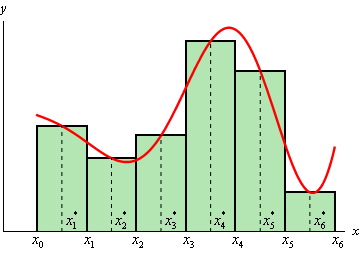
\includegraphics[width=0.4\linewidth]{approx-rectangles}
\end{center}
We start with the simplest and most naive approximation: using a bunch of rectangles under the curve. Suppose
we wish to find the area under the curve $ y = f(x) $ between the two lines $ x = a $ and $ x = b $ by splitting
it up into $ n $ rectangles of width $ \Delta x $. If we pick a value $ x_i^\ast $ inside each rectangle, as shown
in the diagram, the approximate area is
\begin{displaymath}
  f(x_1^\ast) \Delta x + \cdots + f(x_n^\ast) \Delta x = \sum_{i = 1}^n f(x_i^\ast) \Delta x.
\end{displaymath}

Usually, we pick each $ x_i^\ast $ to be either the left-hand or right-hand edge of each rectangle. Note that
we also have $ \Delta x = \frac{b - a}{n} $ and so our left-hand approximation becomes
\begin{displaymath}
  L_n = \frac{b - a}{n} \left[ f(x_0) + \cdots + f(x_{n - 1}) \right]
\end{displaymath}
and the right-hand approximation is
\begin{displaymath}
  R_n = \frac{b - a}{n} \left[ f(x_1) + \cdots + f(x_{n}) \right].
\end{displaymath}

\subsection*{Approximating area using trapezoids}
\begin{center}
  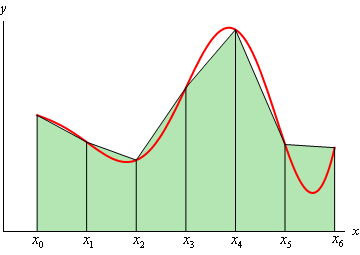
\includegraphics[width=0.4\linewidth]{approx-trapezoids}
\end{center}
A more useful approximation is found when we inscribe trapezoids into the curve. This can be done by taking
the average of the left-hand and right-hand rectangle approximations (recall that the area of a trapezoid is
the average of the area of two rectangles). When we do this, we obtain
\begin{displaymath}
  T_n = \frac{b - a}{2n} \left( f(x_0) + f(x_n) + 2\left[f(x_2) + \cdots + f(x_{n - 1})\right] \right).
\end{displaymath}

\subsection*{Approximating area using parabolae}
\begin{center}
  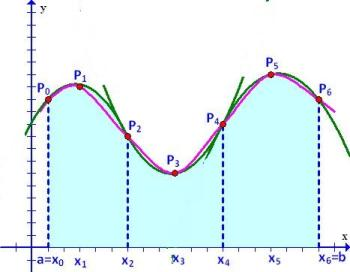
\includegraphics[width=0.4\linewidth]{approx-parabolae}
\end{center}
An even better approximation (for smooth functions) is formed when we use parabolae to estimate the area. The
resulting formula is called \textbf{Simpson's rule}. Note that $ n $ must be even to use Simpson's rule.
\begin{displaymath}
  S_n = \frac{b - a}{3n} \left( f(x_0) + f(x_n) + 4\left[f(x_1) + f(x_3) + \cdots + f(x_{n - 1})\right] + 2\left[ f(x_2) + \cdots + f(x_{n - 2}) \right] \right).
\end{displaymath}

\subsection*{The Definite Integral}
It is obvious that all three methods of approximating area above will approach the `real' area of the curve as $ n \to \infty $. We
call the true area under a curve $ y = f(x) $ from $ x = a $ to $ x = b $ the \textbf{definite integral} of the curve from $ a $ to $ b $,
and we notate it as\footnote{Technically, this is the \textbf{Riemann integral}; there are other kinds of integral.}
\begin{displaymath}
  \lim_{n \to \infty} R_n = \lim_{n \to \infty} L_n = \lim_{n \to \infty} T_n = \lim_{n \to \infty} S_n = \rint^b_a f(x) \dif{x}.
\end{displaymath}

The large $ \rint $ is an elongated `S', which stands for \textit{sum} --- we are summing all of the little areas from $ a $ to $ b $.
Note the similarity to the notation above: we replace $ \sum $ with $ \rint $, $ x_i^\ast $ with $ x $, and $ \Delta x $ with $ \dif{x} $.

The $ \dif{x} $ is \textit{not a number}; it is merely a piece of notation which tells us which variable we are taking area with respect to.
For example, $ \rint^b_a x^2 + y^3 \dif{x} \neq \rint^b_a x^2 + y^3 \dif{y} $. At this stage in time, you can think of the notation as a
pair of fancy brackets: the $ \rint^{z_1}_{z_0} $ corresponds to $ \big( $, and the $ \dif{z} $ corresponds to $ \big) $. It makes no
sense to have one without the other (or, for that matter, to have $ \rint $ without the bounds).

\clearpage
\subsection*{Questions}
\begin{questions}
  \questioA Estimate the area under the graph of $ f(x) = \cos x $ from $ x = 0 $ to $ x = \frac{\pi}{2} $ using four approximating
            rectangles and right endpoints. Sketch the graph and the rectangles. Is your estimate an overestimate or an underestimate?
  \questioA Estimate the area under the graph of $ f(x) = \sqrt x $ from $ x = 0 $ to $ x = 4 $ using four approximating
            rectangles and left endpoints. Sketch the graph and the rectangles. Is your estimate an overestimate or an underestimate?
  \questioA Using the trapezoidal rule with $ n = 4 $, estimate the area under the graph of $ f(x) = 1 + x^2 $ from $ x = -1 $ to $ x = 2 $.
            Repeat with $ n = 8 $. Compare the two results.
  \questioA Use Simpson's rule with $ n = 10 $ to estimate the area under the graph of $ y = e^{x^2} $ from $ x = 0 $ to $ x = 1 $.
  \questioA Use both the trapezoidal rule and Simpson's rule (both with $ n = 10 $) to compute the area under the graph of $ y = \sqrt{z} e^{-z} $
            from $ z = 0 $ to $ z = 1 $.
  \questioA Using four rectangles, find the approximate area under the the graph of $ f(x) $ from $ x = 1 $ to $ x = 5 $ given the following table.
            \begin{center}
              \begin{tabular}{|c|c||c|c|}\hline
                $ x $ & $ f(x) $ & $ x $ & $ f(x) $\\\hline
                1.0 & 2.4 & 3.5 & 4.0\\
                1.5 & 2.9 & 4.0 & 4.1\\
                2.0 & 3.3 & 4.5 & 3.9\\
                2.5 & 3.6 & 5.0 & 3.5\\
                3.0 & 3.8 &&\\\hline
              \end{tabular}
            \end{center}
  \questioM Find the area of a circle of radius 4 using Simpson's rule with $ n = 4 $. What is the percentage error of the estimate?
  \questioA Approximate the area under $ y = f(x) $ from $ x = 0 $ to $ x = 6 $ using Simpson's rule.
            \begin{center}
              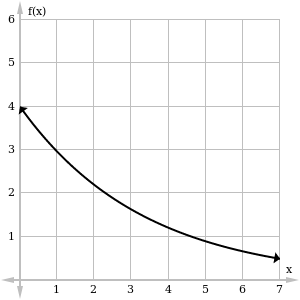
\includegraphics[width=0.35\linewidth]{aa1}
            \end{center}
  \clearpage
  \questioA Approximate the area under $ y = f(x) $ from $ x = 0 $ to $ x = 10 $ using the trapezoidal rule.
            \begin{center}
              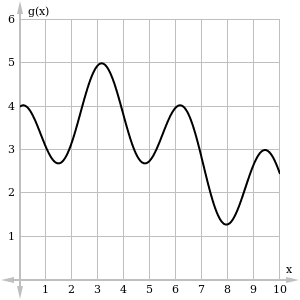
\includegraphics[width=0.35\linewidth]{aa2}
            \end{center}
  \questioM Approximate the shaded area using the trapezoidal rule.
            \begin{center}
              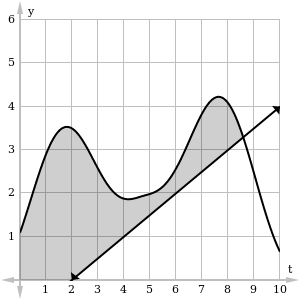
\includegraphics[width=0.35\linewidth]{aa3}
            \end{center}
  \questioM Show that $ T_n = \frac{1}{2} (L_n + R_n) $.
  \questioA (Lifted straight from a Level 2 worksheet.)
    \begin{parts}
      \part Draw the line $ y = 2t + 1 $ and use geometry to find the area under
            this line, above the $ t$-axis, and between the vertical lines $ t = 1 $
            and $ t = 3 $ (i.e. find $ \rint_1^3 2t + 1 \dif{t} $ using geometry).
      \part If $ x > 1 $, let $ A(x) $ be the area of the region that lies under the line $ y = 2t + 1 $
            between $ t = 1 $ and $ t = x $. Sketch this region and use geometry to find an expression
            for $ A(x) $ (i.e. find $ A(x) = \rint_1^x 2t + 1 \dif{t} $ using geometry).
      \part Find $ A'(x) $. What do you notice?
    \end{parts}
\end{questions}

\end{document}
